%todo: complete, this is what my program does
In this chapter we will discuss the architecture of our framework and the tools used for this thesis in Deception Detection. We will introduce the OpenFace toolkit (\ref{OpenFace}), and describe landmark detection (\ref{landmark_det}), action unit recognition (\ref{au_det}) and the deception detection process (\ref{dec_det}).

\section{General Architecture}
%todo with images + change title
The general idea of this thesis is to classify whether a person is telling the truth or lying, by analyzing the subject's facial movement, extracted using an RGB camera, during a video. To achieve this it is fundamental that the subject's face results visible during the videos.

We implemented this idea using a Support Vector Machine classifier. 

The architecture utilized is shown in fig \ref{fig:architecture} and is composed this way:

\begin{itemize}
	\item We gather a video of a person in a high stake situation.
	\item Detect the face of the person in the video using Constrained Local Neural Field.
	\item Detect the facial landmarks using Convolutional Experts Network.
	\item Extract the appearance features in the form of Histogram of Oriented Gradients and perform dimensionality reduction and feature normalization through Principal Component Analysis.
	\item Extract action unit presence and intensity from the videos using a SVM.
	\item Feed the extracted data to train an SVM for classification on a test set.
\end{itemize}

\clearpage

\section{OpenFace} \label{OpenFace}
The OpenFace \cite{Baltru2018} toolkit is a tool for machine learning and computer vision researchers, created by Baltrusaitis et al., to support performing facial landmark detection, head pose estimation, action unit recognition, feature extraction and eye gaze estimation. 

\begin{figure}[H]
	\centering
	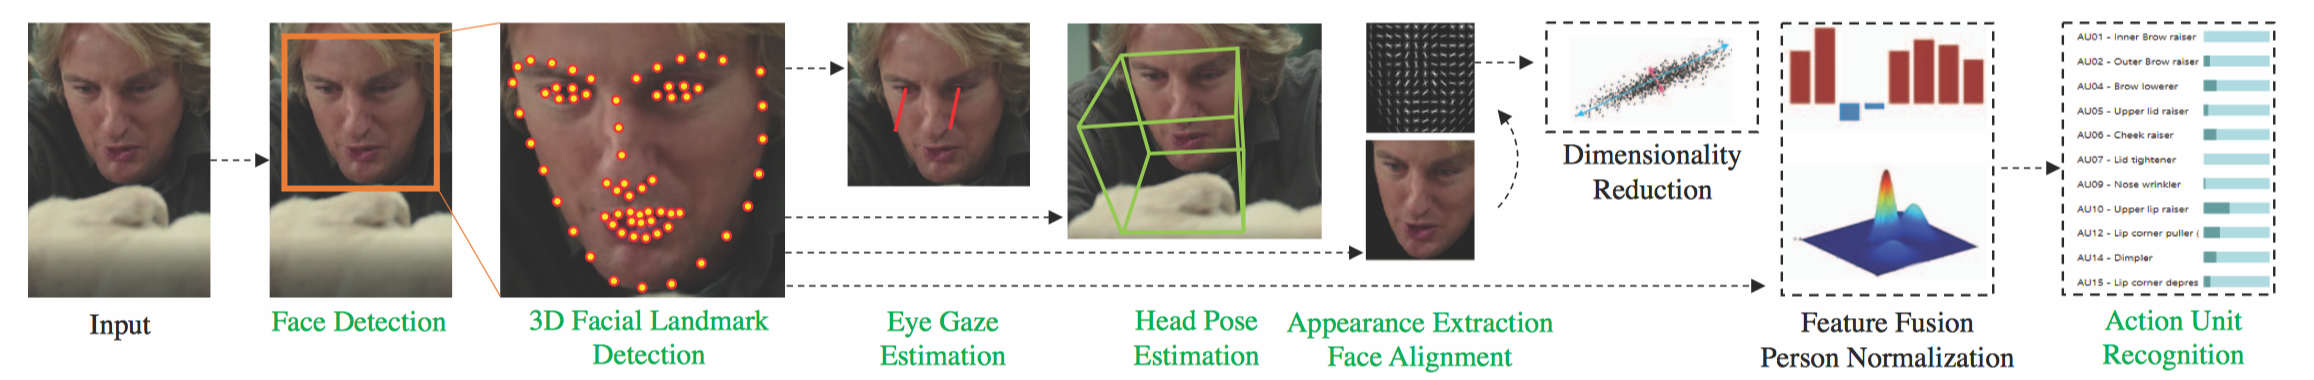
\includegraphics[width=1\textwidth]{openface20_pipeline}
	\caption{OpenFace Pipeline \cite{Baltru2018}}
	\label{fig:openface20_pipeline}
\end{figure}

%TODO: check this new addition
This tool is customizable in the way that all the SVM models and neural networks can be trained with new datasets, and the code is open source, so it can be changed to fit the needs of the experimenters.


\clearpage

\section{Landmark Detection} \label{landmark_det}

The first step in Action Unit identification is to detect the facial landmarks. To accomplish this a local detector called Convolutional Experts Network (CEN) (Fig. \ref{fig:CEN}) is utilized. 

CEN has the advantage of aggregating a neural architecture and patch experts (local detectors, they evaluate the probability of a landmark being aligned at a particular pixel location). CEN can learn different patch experts and adapt to diverse appearance models without explicitly labeling attributes.

\begin{figure}[H]
	\centering
	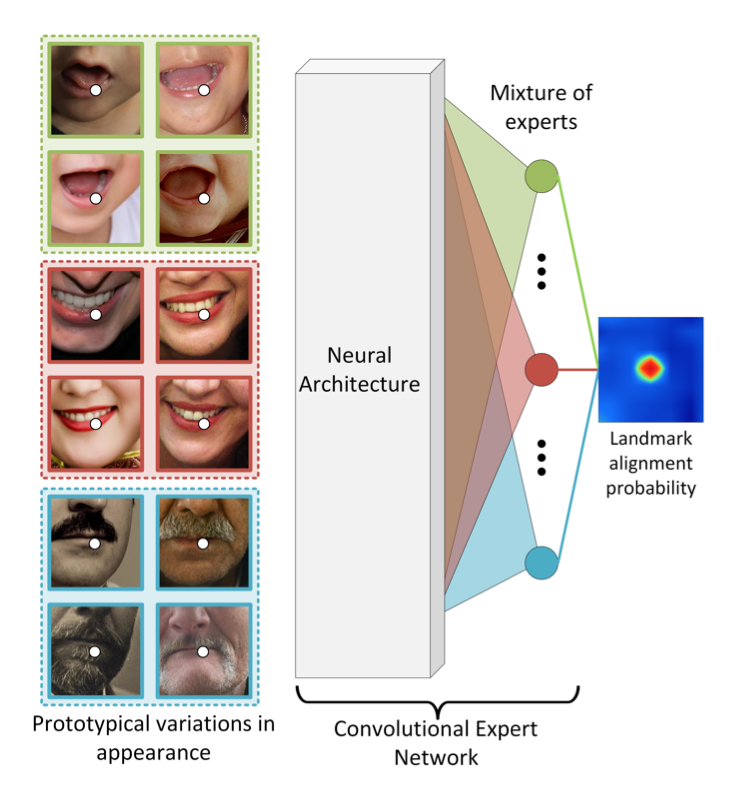
\includegraphics[width=0.75\textwidth]{CEN}
	\caption{Facial landmarks naturally cluster around appearance prototypes (facial hair, expressions, make-up etc). To model such appearance variations a Convolutional Experts Network is used to merge the advantages of neural architectures and mixtures of patch experts, to model landmark alignment probability \cite{Baltru2017}.}
	\label{fig:CEN}
\end{figure}

%TODO: write better?
OpenFace uses a Convolutional Experts Constrained Local Model (CE-CLM) \cite{Baltru2017}, which is a Constrained Local Model (CLM) that uses CEN as a local detector. 

A Constrained Local Model is class of methods for locating sets of points (constrained by a statistical shape model) on a target image \cite{clm_cootes}.

Generally the procedure is as follows (Fig. \ref{fig:CLM}):
\begin{itemize}[noitemsep]
	\item Sample a region from the image around the current estimate, projecting it into a reference frame.
	\item For each point, generate a "response image" giving a cost for having the point at each pixel.
	\item Search for a combination of points which optimizes the total cost, by manipulating the shape model parameters.
\end{itemize}

%todo: pic from https://pdfs.semanticscholar.org/c2a3/850becae2799b0e591e7ab1008b84897d6e9.pdf
\begin{figure}[H]
	\centering
	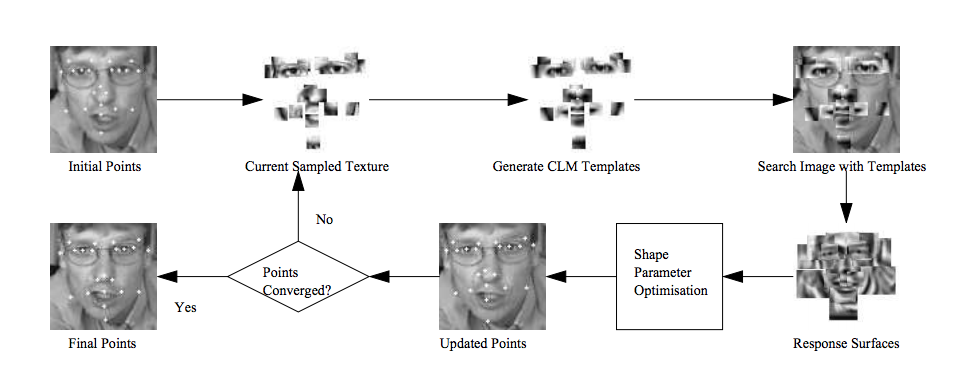
\includegraphics[width=1\textwidth]{CLM}
	\caption{Overview of CLM \cite{clm_cootes}.}
	\label{fig:CLM}
\end{figure}

CLM are used to model the appearance of each facial landmark individually by using local detectors and a shape model for constrained optimization. 

The CE-CLM is divided in two fundamental parts: response map computation using CEN, and shape parameter update.

In the first step, the landmarks alignment is computed separately from the other landmarks. \\
In the second phase, all landmarks are considered together and for misaligned landmarks and irregular shapes their position is penalized, using a Point Distribution Model (PDM).

\subsection{CEN}
In the initial step, the objective is to generate a response map to localize the individual landmarks. This is performed by assessing the landmark alignment probability at specific pixel locations. \\
CEN takes in input a Region of Interest (ROI) around the currently estimated position of a landmark, and outputs a response map that calculates the landmark alignment probability at each pixel location (Fig. \ref{fig:landmark_det}).

\begin{figure}[H]
	\centering
	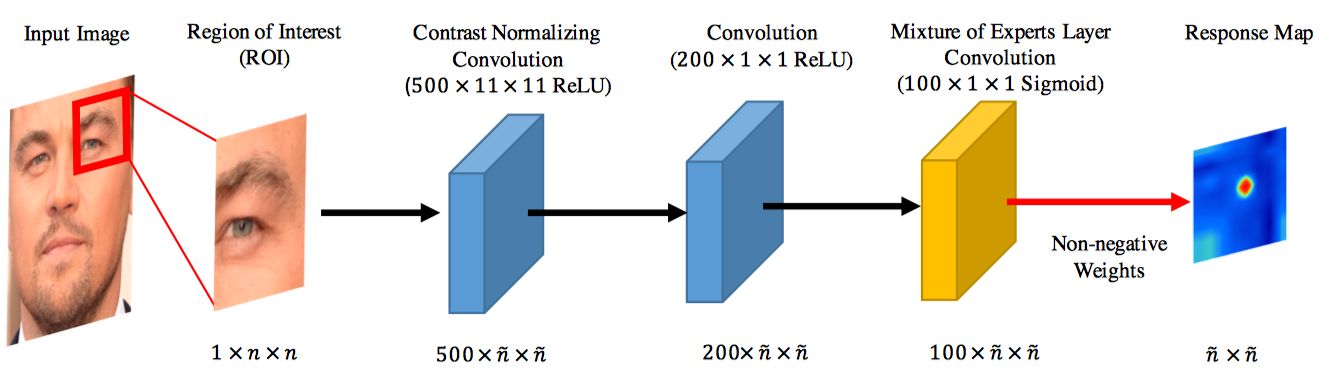
\includegraphics[width=1\textwidth]{landmark_det}
	\caption{Overview of the Convolutional Experts Network model. The output response map is a non-negative and non-linear combination of neurons in ME-layer using a sigmoid activation \cite{Baltru2017}.}
	\label{fig:landmark_det}
\end{figure}

%TODO: to specific?
In order to do all this, the ROI is initially passed in a Contrast Normalizing Convolution layer to perform z-score normalization and to calculate the correlation between input and kernel. The output is then convolved in another layer of ReLU neurons (convolution is an operation on two functions to produce a third function that expresses how the shape of one is modified by the other).

The last neural layer before the response map is the Mixture of Expert Layer (ME-layer), and it can model the alignment probability using a combination of patch experts (local detectors) that are able to represent different landmarks appearance prototypes by outputting individual votes on alignment through a sigmoid function. The response maps from all the local detectors are then combined in the last layer, giving the final alignment probability.

\subsection{Point Distribution Model}
%TODO: from wiki modify a bit
The Point Distribution Model is a used to represent the mean geometry of a shape and some statistical modes of geometric variation inferred from a training set of shapes \cite{wiki:PDM}. 

\begin{figure}[H]
	\centering
	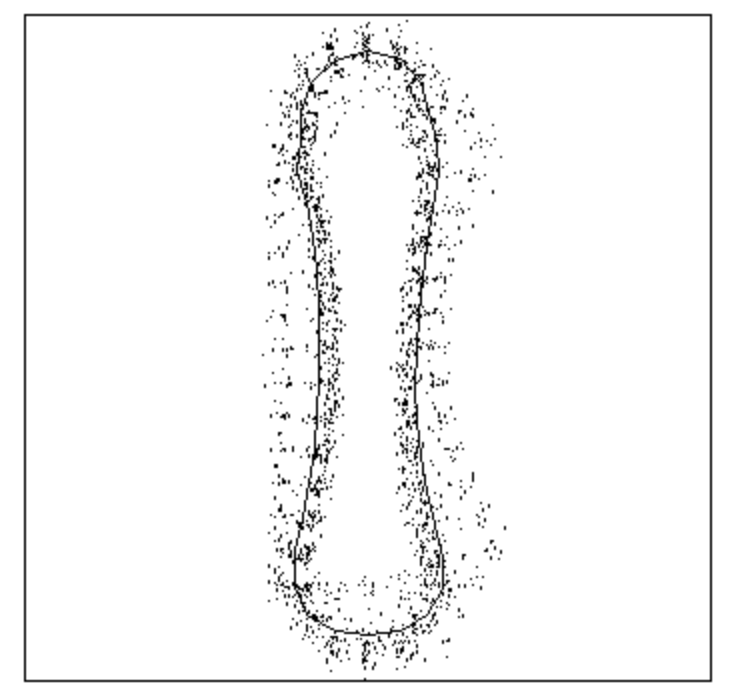
\includegraphics[width=0.45\textwidth]{PDM}
	\caption{PDM of a metacarpal. Dots mark the possible position of landmarks, and the line denote the mean shape \cite{PDM}.}
	\label{fig:PDM}
\end{figure}

Point distribution models rely on landmark points. The general PDM works this way:
\begin{enumerate}
	\item A set of training images are manually landmarked to sufficiently approximate the geometry of the original shapes. 
	\item This \textit{k} landmarks are aligned in two dimensions resulting in \\
	$\mathbf{X} = (x_1,y_1, \dots, x_k, y_k)$
	\item The shape outlines are reduced to sequences of k landmarks, so that any given training shape can be defined by the vector $\mathbf{X} \in {\mathbb{R} ^{2k}}$.
	\item The matrix of the top $d$ eigenvectors is given as $\mathbf{P} \in \mathbb{R}^{2k \times d}$, and each eigenvector describes a principal mode of variation along the set.
	\item A linear combination of the eigenvectors is used to define a new shape $ \mathbf{X} '$, mathematically defined as: 
	\begin{equation}
	\mathbf {X}' = {\overline {\mathbf {X}} + \mathbf{P} \mathbf{b}}
	\end{equation}
	
	where $ {\overline {\mathbf {X}}}$ is defined as the mean shape across all training images, and $\mathbf {b}$ is a vector of scaling values for each principal component. 
	\item By modifying the variable $\mathbf {b}$  an infinite number of shapes can be defined. $\mathbf {b}$ shouldn't generally be modified more than $\pm3\sigma$ \cite{wiki:PDM}.
\end{enumerate}

With the OpenFace framework Point Distribution Model \cite{PDM_RLMS} we model the location of facial feature points in the image, using non-rigid shape and rigid global transformation parameters.

The application of PDM has two objectives:

\begin{itemize}
	\item They are employed to control the landmark locations.
	\item They are used to regularize the shapes in the CE-CLM framework by using Non-Uniform Regularized Landmark Mean Shift (NU-RLMS) \cite{Baltru2013}.
\end{itemize}
This has an effect in the final detected landmarks, where the irregular shapes are imposed a penalty.

The results can be seen in the figure \ref{fig:land_det_ex} below for different images with different illuminations and angles. 

\begin{figure}[H]
	\centering
	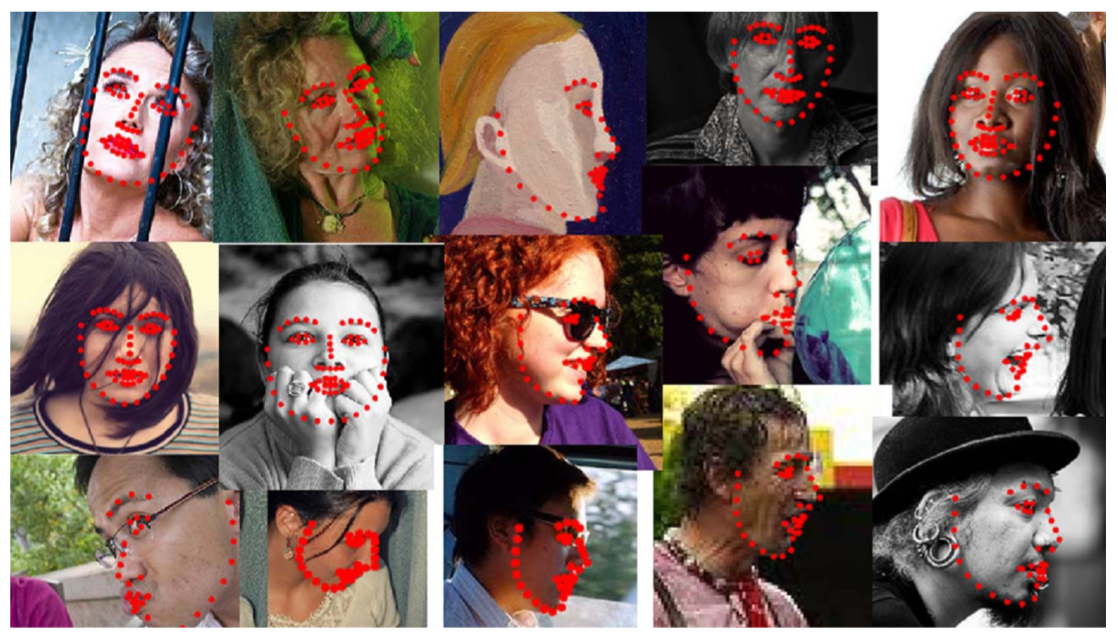
\includegraphics[width=0.85\textwidth]{land_det_ex}
	\caption{Example of different facial landmarks detected in diverse conditions and viewing angles. \cite{Baltru2018}.}
	\label{fig:land_det_ex}
\end{figure}

\clearpage

\section{Action Unit Detection} \label{au_det}
Action Unit (AU) detection plays a fundamental role in our work. We now describe the process used to detect the AUs through an SVM, starting with an overview of the datasets utilized for training the SVM in AUs detection.

\begin{figure}[H]
	\centering
	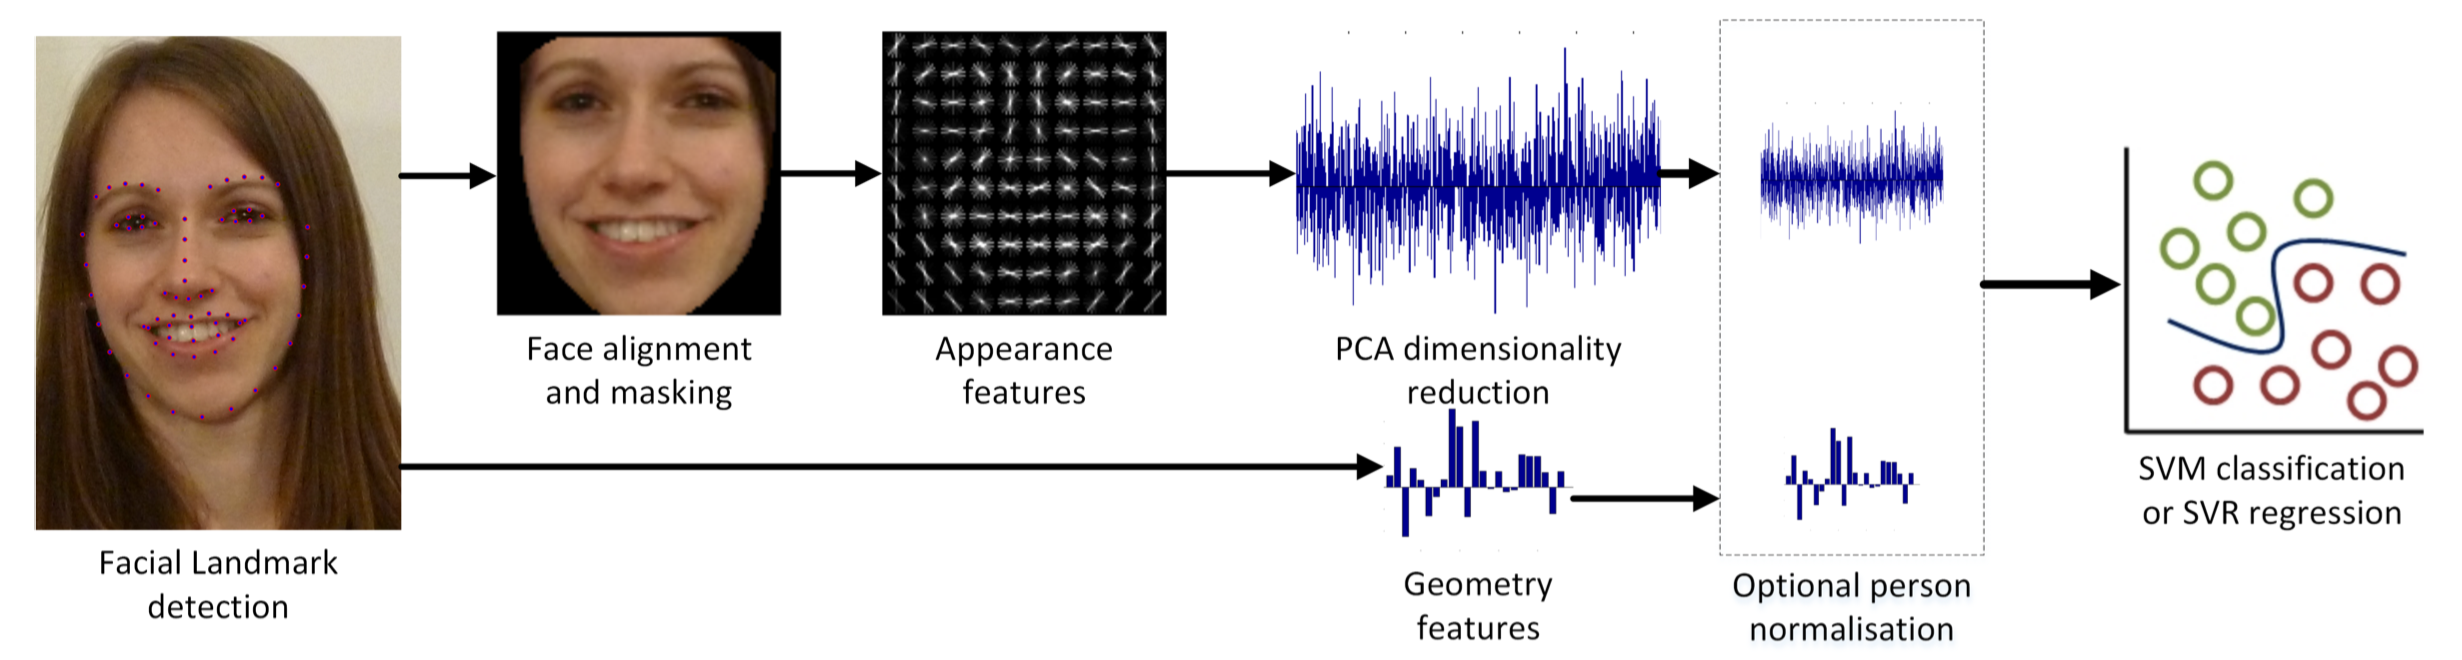
\includegraphics[width=1\textwidth]{AU_pipeline}
	\caption{AU detection and intensity pipeline \cite{Baltru2015}.}
	\label{fig:AU_pipeline}
\end{figure}

\subsection{Training Datasets}
%todo: this part might not be necessary here? I could expand a lot on it in the experiments section
There are four main dataset used for training the Action Unit detection system: DISFA \cite{DISFA}, BP4D-Spontaneous \cite{BP4D-Spontaneous}, SEMAINE \cite{SEMAINE} and CK+ \cite{CK+}. These four datasets consist of videos of people subject to emotion inducing tasks.

The \textbf{BP4D} database of spontaneous facial expressions includes videos of 41 participants (23 women and 18 men, 21 for training and 20 for validating). The age ranged from 18 to 29; 11 were Asian, 6 African-American, 4 Hispanic, and 20 Euro-American. \\
Emotion inducing techniques were used to elicit an emotional response. Frame-level ground-truth for facial actions was obtained by using the Facial Action Coding System annotations, performed by trained professionals. \\
Each participant in the database is associated with 8 tasks. For each task, there are both 3D and 2D videos and the metadata include annotations for 11 AUs for occurrence and 5 AUs for intensities.

\textbf{DISFA} (Denver Intensity of Spontaneuos Facial Action) Database is a non posed facial expression database for automatic action unit detection. It contains videos of 27 participants (12 female, 15 males; 14 used for training and 13 for validation). It includes 4 minute-long videos of spontaneous facial expression, resulting in 130k frames annotated for 12 AUs (Fig. \ref{fig:DISFA_AU}), comprehensive of AUs intensity on a 0 to 5 scale.

\begin{figure}[H]
	\centering
	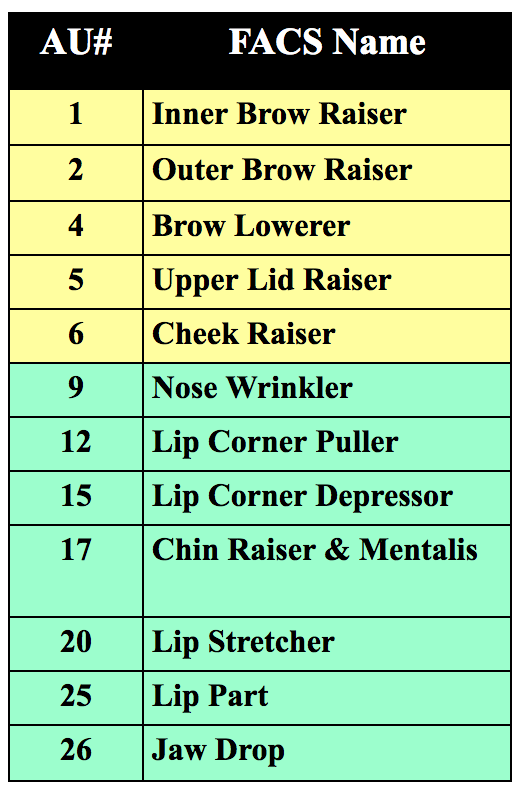
\includegraphics[width=0.5\textwidth]{DISFA_AU}
	\caption{AUs coded in the DISFA database \cite{DISFA_AU}.}
	\label{fig:DISFA_AU}
\end{figure}

The FACS annotated \textbf{SEMAINE} subset contains recordings of 31 subjects (15 for training and 16 for validation). It consists of one minute long recordings, leading to 93k frames labeled for 5 AU occurrences.

The \textbf{Cohn-Kanade} AU-Coded Facial Expression Database is utilized for research in facial image analysis. \\
CK+, includes both posed and non-posed (spontaneous) expressions and additional types of metadata. Each posed expression is completely FACS coded, and emotion labels are part of the metadata. \\
CK+ also provides baseline results for facial feature tracking, action unit and emotion recognition.

BP4D, SEMAINE and DISFA have three AUs in common (2, 12, and 17). \\
SEMAINE and DISFA share AUs 2, 12, 17, 25. \\
BP4D and DISFA share AUs 1, 2, 4, 6, 12, 15, 17. \\
This allows for cross-dataset training.

By training on these dataset is possible to detect the following AUs (\ref{fig:all_AUs}):

\begin{figure}[H]
	\centering
	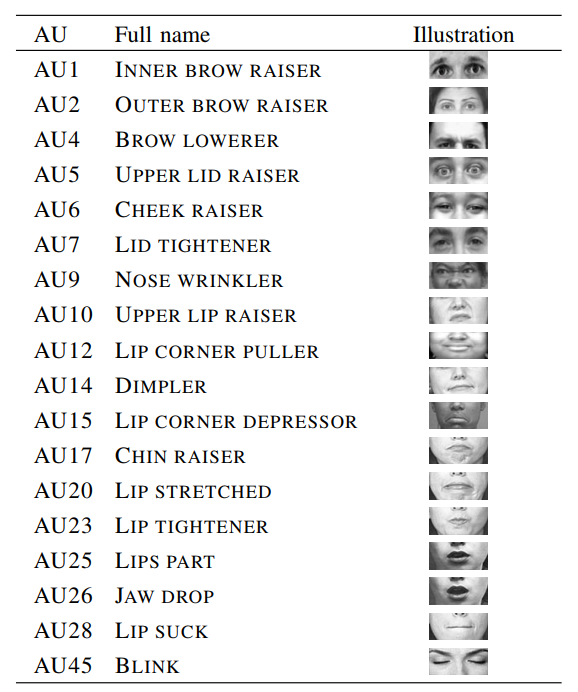
\includegraphics[width=0.85\textwidth]{all_aus}
	\caption{List of available AUs for prediction \cite{Baltru2018}.}
	\label{fig:all_AUs}
\end{figure}

\subsection{Feature Extraction}
There are two types of features that are used: appearance (Histogram of Oriented Gradients) and geometry (shape parameters and landmark locations) ones. To extract those features it's required to track certain landmarks on the face, and then continue this process by performing face alignment.

\subsubsection{Face Tracking}
%TODO: rewrite
Face tacking is done by utilizing Constrained Local Neural Field (CLNF) facial landmark detector and tracker, backed up by a structural SVM for facial detection \cite{Baltru2013}.
CLNF is a specific case of Constrained Local Model (CLM), that differs from the original by utilizing more advanced local detectors and a different optimization function.

The Constrained Local Model can be described by the following parameters: \\
$p = [s, \mathbf{R}, \mathbf{p}, \mathbf{t}]$.
\begin{itemize}[noitemsep, topsep = -5pt]
	\item \textit{s} is the scale factor.
	\item \textbf{R} is the object rotation.
	\item \textbf{t} is the 2D translation.
	\item \textbf{p} describes the shape of a vector of non rigid variations.
\end{itemize}

These parameters can be modified to compute different versions of the model. The resulting point distribution model is:

\begin{equation} \label{eq:pdm}
	x_i = s \cdot \mathbf{R}(\overline{x_i} + \phi_i \mathbf{p}) + \mathbf{t}
\end{equation}

Where $x_i$ is the location of the i\textit{th} feature point in an image, $\overline{x_i}$ is the mean of the i\textit{th} element of the PDM, and $\phi_i$ is the i\textit{th} eigenvector that describes the variation of the feature point.

In the Constrained Local Model we use the parameters from face detection to estimate the maximum a posteriori probability \textit{p} of the face model.

\subsubsection{Alignment and Masking}
For the extracted face to be correctly analyzed, there needs to be a mapping to a common reference frame, and the changes resulting from scaling and in plane rotation needs to be removed. 

In order to achieve this, a similarity transform from the currently detected landmarks to a representation of frontal landmarks from a neutral expression (projection of mean shape from a 3D PDM) is utilized. \\
The similarity transform is done with Procrustes superimposition that minimizes the mean square error between aligned pixels \cite{Baltru2013}.\\
The result is a $112 \times 112$ pixel image of the face with 45 pixel interpupillary distance (Fig \ref{fig:alignment_masking}). 

To reduce the weight of significant facial expressions (mouth opening, brow raises etc.) on the similarity transform, only the most stable facial landmarks must be used. \\
%TODO: non mi piace
In order to determine those points, the most stable CLNF detected landmarks on the CK+ dataset \cite{CK+} are examined.

\begin{figure}[H]
	\centering
	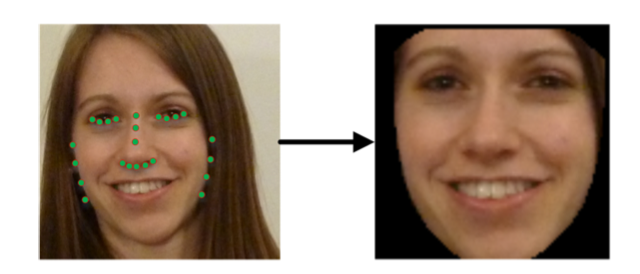
\includegraphics[width=0.75\textwidth]{alignment_masking}
	\caption{Stable points used for alignment to a common reference frame, followed by masking \cite{Baltru2015}.}
	\label{fig:alignment_masking}
\end{figure}

Masking, performed using a convex hull surrounding the feature points, is done to remove informations from the image that do not regard the face.

\subsubsection{Appearance Features}
After the face is aligned to a $112 \times 112$ image it's time to extract the appearance features. \\
To get the appearance features, $12 \times 12$ block of 31 dimensional Histogram of Oriented Gradients (HOG) are extracted, giving a 4464 dimensional vector characterizing the face. The implementation for HoG comes from dlib \cite{dlib}.

Once the feature vector is obtained, the next step is to reduce it's dimensionality. In order to do that Principal Component Analysis (PCA) is applied. \\
To generalize the dimensionality reduction, the training was performed on the FERA 2015 \cite{FERA15}, CK+ \cite{CK+}, DISFA \cite{DISFA}, AVEC 2011 \cite{AVEC11} and FERA 2011 \cite{FERA11} datasets. \\
By using PCA while sub-sampling from peak and neutral expressions and keeping 95\% of explained variability, the feature vector becomes of 1379 dimensions.

\subsubsection{Geometry Features}
%TODO: CHECK CLNF STUFF
The geometry features are obtained trough the CE-CLM models, and consist of non-rigid shape parameters and landmarks locations ($p$ and $ \phi_i p$ in equation \ref{eq:pdm}). this results in a 227 dimensional vector representing geometry features.\\
Summed to the appearance features, this leads to a 1606 dimensional vector that defines the appearance of the face.

\subsubsection{Neutral Expression Extraction}
To extract some of the facial expression is very important to have a neutral starting expression. There are personal differences on how we appear while in a neutral resting state, such as people looking naturally more cheerful or sad then others \cite{normexpr}. To address this issue there needs to be a person specific calibration, done by adjusting for neutral expressions \cite{Baltru2013}.

Neutral expression adjustments are done by computing the median value of the face descriptors in a video, leading to a neutral expression descriptor. This works assuming that in a video most of the frames will contain a neutral expression, and this should hold true especially for real life situations where most of the time the interactions are performed with a neutral expression \cite{NatAffData}.

Once the neutral descriptor is computed, it is subtracted from the feature descriptor, giving normalized features. 
%To help with the ease of computing the median, a histogram is kept for each element in the feature vector.

\subsubsection{Classification and Regression}
The next step is to extract Action Units from each frame of the video. Both intensity and presence are extracted.

Action Units detection is performed through Support Vector Machines (SVM), and Action Unit intensity using Support Vector Regression (SVR), both using the liblinear implementation \cite{liblinear}. In both cases a linear kernel is utilized, as more complex kernels had no effect on performances and were quite slower to train.  

Since the AU occurrences are not balanced by nature (for example AU28, blinking, is not very frequent if we analyze each frame of a video), it's highly important to balance the training data. To do this it was needed to undersample the negative AU samples from training data, thus getting to an equal number of positive and negative samples.

\clearpage

\section{Deception Detection} \label{dec_det}
%TODO: rewrite, tentative
In this step we feed the extracted action units from the videos to an SVM for classification.
We use an SVM because after a lot of testing with different techniques that was the one that performed the best compared to others. 

%todo: come prendiamo i dati, cosa facciamo... 
\subsection{Data pre-processing}
Before feeding the videos to the SVM for Action Units extraction we had to make sure the videos were in good enough condition to be processed. That is not given since all this videos come from real life trials and the recording conditions are not optimal.

Being in an acceptable condition means that the face should be clearly visible, and the video has to have the specific person visible and talking in \textit{most} of the video, and no other people on it, so to avoid training on different subjects of which we are not sure if they are lying or telling the truth.

As a consequence many videos had to be cut, trimmed or discarded to reach an acceptable level.

After extracting Action Units intensity and presence from our dataset of videos (\ref{rldb}) we put the data in a \textit{csv} format to be able to pass them to the SVM. 

The data are divided for both AUs intensity, ranging from $0$ to $5$, and AU presence, having the boolean value of either $0$ or $1$ if the AU was missing or present in the specific frame of the video.

\begin{figure}[H]
	\centering
	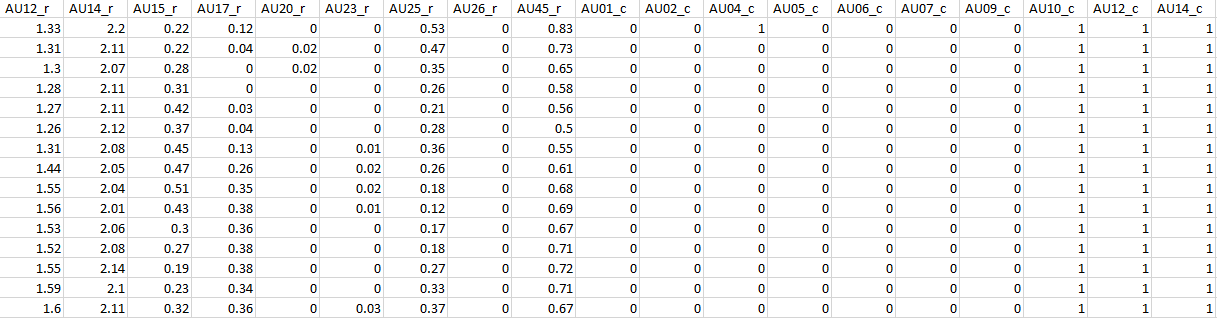
\includegraphics[width=1\textwidth]{dataset_csv}
	\caption{Example of input data in csv format.}
	\label{fig:dataset_csv}
\end{figure}

The next step is to remove all the rows that have both no intensity and no presence for AUs, since those rows are most likely errors from the extraction, deriving from the poor quality of the videos.

%todo: forse non e' utile qui ma in generale lo devo dire
We organized the data in three sets, one concerning only AUs intensity, one with only AUs presence, and another one where we merged the previous ones together, in order to better analyze the data and understand it's structure.

\subsection{SVM}
%todo: svm personalizzato a quello che ho fatto


